\documentclass[a4paper]{article}

%use the english line for english reports
%usepackage[english]{babel}
\usepackage[portuguese]{babel}
\usepackage[utf8]{inputenc}
\usepackage{indentfirst}
\usepackage{graphicx}
\usepackage{verbatim}


\begin{document}

\setlength{\textwidth}{16cm}
\setlength{\textheight}{22cm}

\title{\Huge\textbf{Título do Trabalho}\linebreak\linebreak\linebreak
\Large\textbf{Relatório Final}\linebreak\linebreak
\linebreak\linebreak

\includegraphics[scale=0.1]{feup-logo.png}\linebreak\linebreak
\linebreak\linebreak
\Large{Mestrado Integrado em Engenharia Informática e Computação} \linebreak\linebreak
\Large{Programação em Lógica}\linebreak
}

\author{\textbf{Grupo 04:}\\ João Nuno Fonseca Seixas - 201505648 \\ Renato Alexandre Sousa Campos - 201504942 \\\linebreak\linebreak \\
 \\ Faculdade de Engenharia da Universidade do Porto \\ Rua Roberto Frias, s\/n, 4200-465 Porto, Portugal \linebreak\linebreak\linebreak
\linebreak\linebreak\vspace{1cm}}
%\date{Junho de 2007}
\maketitle
\thispagestyle{empty}

%************************************************************************************************
%************************************************************************************************

\newpage

\section*{Resumo}
Resumo sucinto do trabalho com 150 a 250 palavras (problema abordado, objetivo, como foi o problema resolvido/abordado, principais resultados e conclusões).

\newpage

\tableofcontents

%************************************************************************************************
%************************************************************************************************

%*************************************************************************************************
%************************************************************************************************

\newpage

%%%%%%%%%%%%%%%%%%%%%%%%%%
\section{Introdução}

Descrever os objetivos e motivação do trabalho. Descrever num parágrafo breve a estrutura do relatório.


%%%%%%%%%%%%%%%%%%%%%%%%%%
\section{O Jogo Campo Bello}

Campo Bello é um jogo que pode ser jogado de 2 a 4 jogadores. Tem inspiração no jogo clássico "Resta Um" ou "Peg Solitaire" em Inglês. É um jogo ainda recente, criado em 2017.
Para ganhar, um jogador deve tentar remover todas as suas peças do tabuleiro antes dos adversários.
O tabuleiro consiste em 4 triângulos que rodeiam um diamante central. Os triângulos correspodem às áreas iniciais de cada jogador. As peças são removidas ao saltar:  saltar uma peça nossa causa a remoção da peça que foi saltada; saltar uma peça adversária permite-nos remover uma peça nossa do tabuleiro.
Na variante de apenas 2 jogadores, que vai ser implementada, os jogadores ficam com triângulos opostos e jogam alternadamente.
É também possível executar saltos duplos e triplos numa só jogada.
No fim do jogo cada jogador pontua 1 ponto por cada uma das suas peças fora da área inicial e 3 pontos por cada uma das suas peças dentro da sua área inicial.
O jogador com menos pontos ganha!\linebreak\linebreak
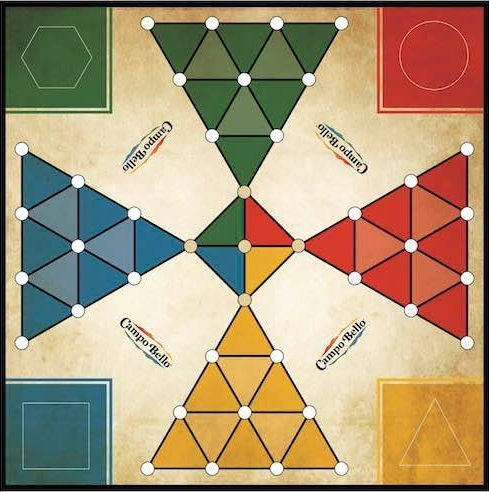
\includegraphics[scale=0.9]{originalBoard.png}\linebreak\linebreak
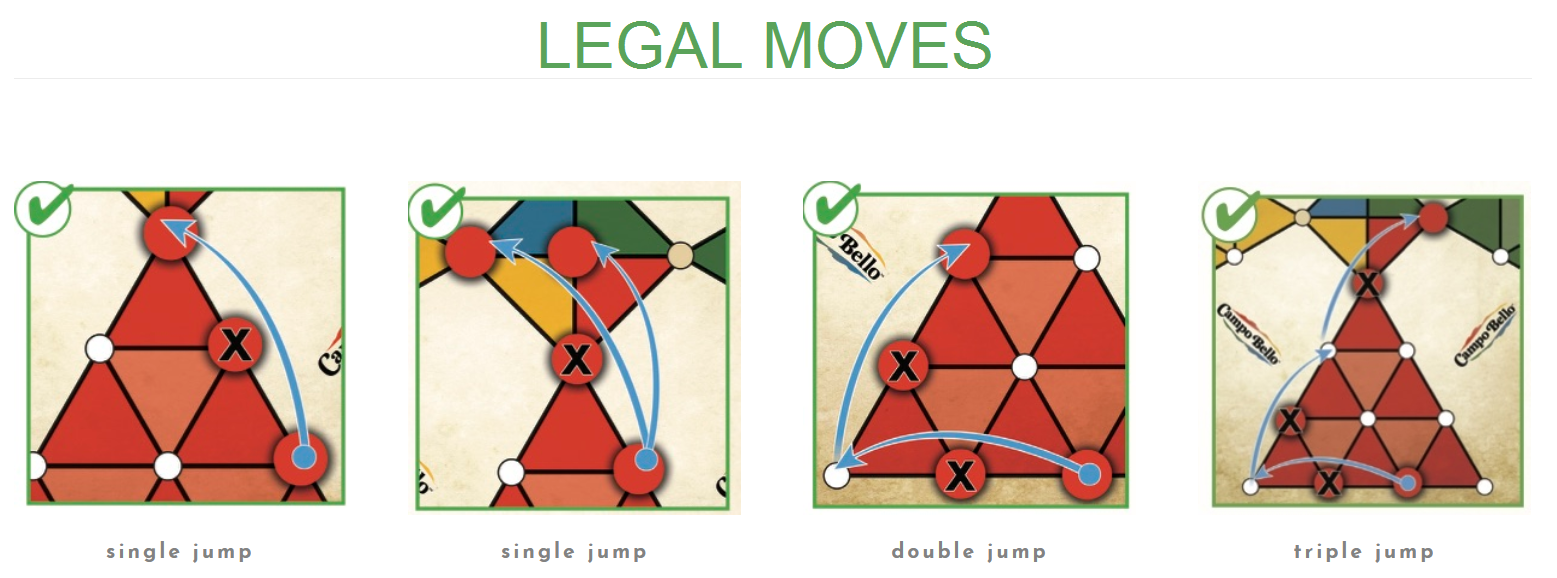
\includegraphics[scale=0.3]{legalMoves.PNG}\linebreak\linebreak
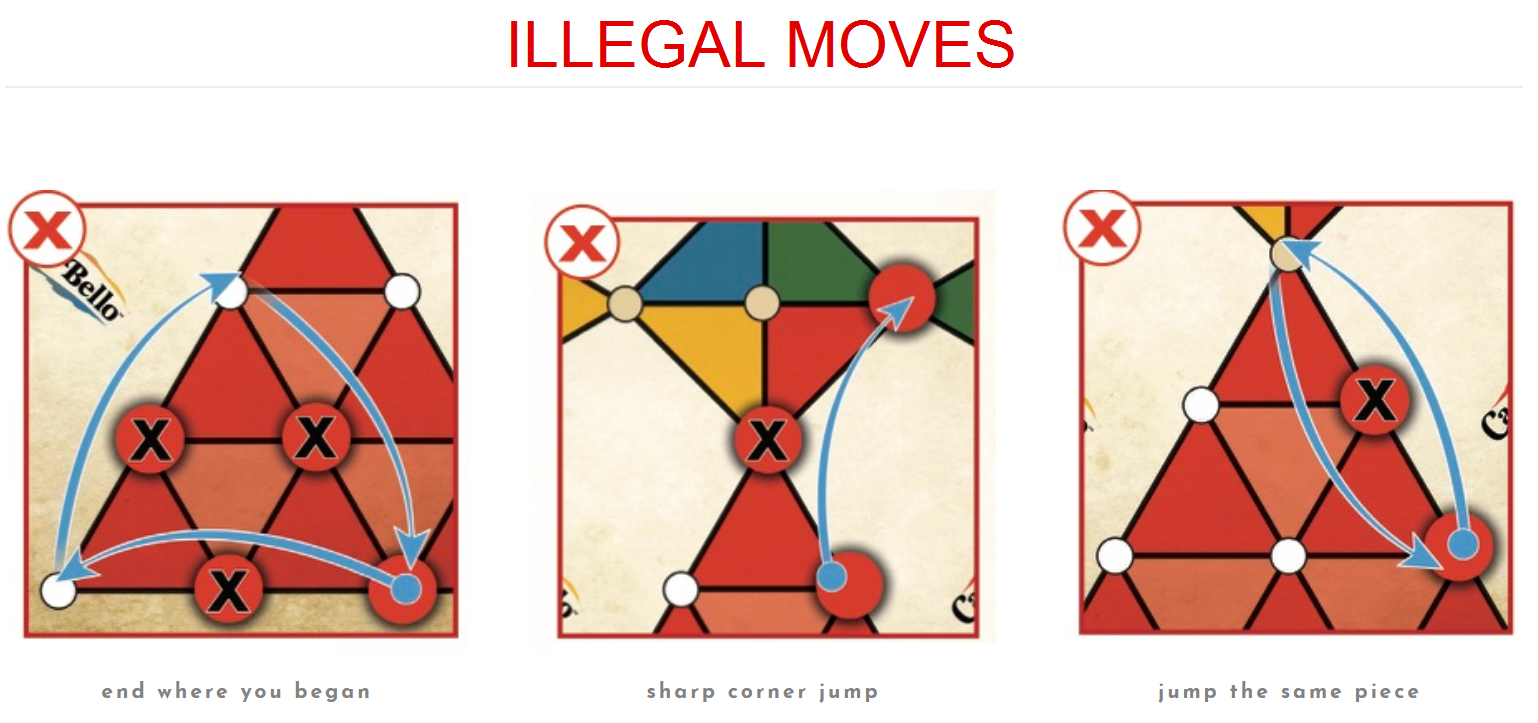
\includegraphics[scale=0.3]{illegalMoves.PNG}\linebreak\linebreak

http://www.campobellogame.com/


%%%%%%%%%%%%%%%%%%%%%%%%%%
\section{Lógica do Jogo}

Descrever o projeto e implementação da lógica do jogo em Prolog, incluindo a forma de representação do estado do tabuleiro e sua visualização, execução de movimentos, verificação do cumprimento das regras do jogo, determinação do final do jogo e cálculo das jogadas a realizar pelo computador utilizando diversos níveis de jogo. Sugere-se a estruturação desta secção da seguinte forma:

\subsection{Representação do Estado do Jogo} O estado do jogo é representado por 2 listas que identificam em que posições do tabuleiro estão as peças de cada jogador (1 lista para cada jogador). As peças de cada jogador sáo designadas em Inglês por "movers".\linebreak
\begin{flushleft} 
Tabuleiro no estado de jogo inicial:
\end{flushleft}
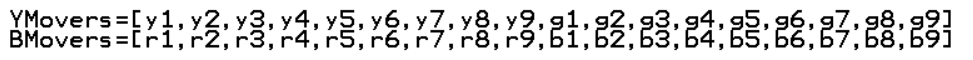
\includegraphics[scale=0.6]{initialBoard.png}\linebreak\linebreak
\begin{flushleft} 
Tabuleiro no estado de jogo intermédio:
\end{flushleft}
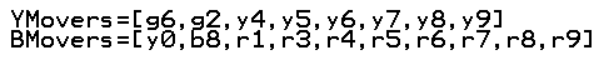
\includegraphics[scale=0.6]{midBoard.png}\linebreak\linebreak
\begin{flushleft} 
Tabuleiro no estado de jogo final:
\end{flushleft}
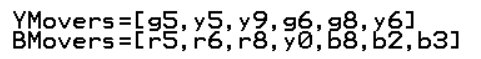
\includegraphics[scale=0.6]{finalBoard.png}\linebreak\linebreak 
Com o decorrer do jogo as listas perdem elementos. O estado final do jogo é alcançado quando uma das listas estiver vazia ou quando não houver mais jogadas possíveis para o jogador que vai jogar.


\subsection{Visualização do Tabuleiro} O predicado para visualização do tabuleiro mostra as posições do tabuleiro do lado esquerdo a usar para os movimentos e do lado direito o estado atual das peças.  Usa \textit{put\_code} para melhorar o aspeto e facilitar a visualição. 

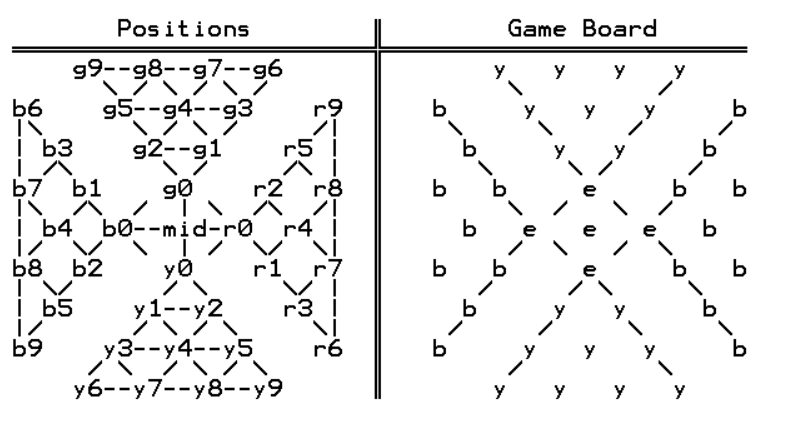
\includegraphics[scale=0.6]{gameBoard.png}\linebreak\linebreak
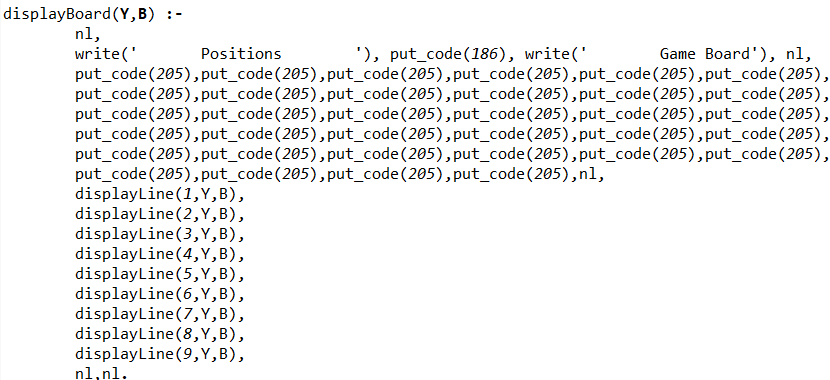
\includegraphics[scale=0.6]{displayBoard.png}\linebreak\linebreak

Estes predicados encarregam-se de imprimir qual a peça do tabuleiro está naquela posição. 

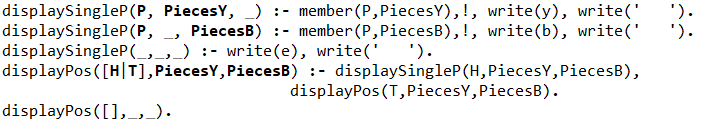
\includegraphics[scale=0.8]{displayBoard1.png}\linebreak\linebreak

O resto é específico de cada linha. Eis o exemplo de uma dessas linhas: 

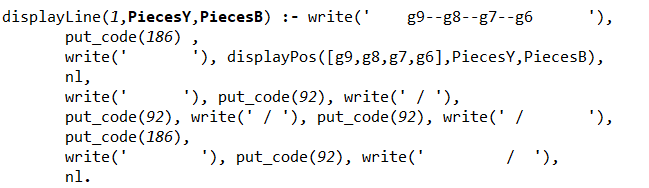
\includegraphics[scale=0.8]{displayBoard2.png}\linebreak\linebreak

\subsection{Lista de Jogadas Válidas} Obtenção de uma lista de jogadas possíveis. Exemplo: \textit{valid\_moves(+Board, -ListOfMoves)}.

\subsection{Execução de Jogadas} Validação e execução de uma jogada num tabuleiro, obtendo o novo estado do jogo. Exemplo: \textit{move(+Move, +Board, -NewBoard)}.

\subsection{Avaliação do Tabuleiro} Avaliação do estado do jogo, que permitirá comparar a aplicação das diversas jogadas disponíveis. Exemplo: \textit{value(+Board, +Player, -Value)}.

\subsection{Final do Jogo} Verificação do fim do jogo, com identificação do vencedor. Exemplo: \textit{game\_over(+Board, -Winner)}.

\subsection{Jogada do Computador} Escolha da jogada a efetuar pelo computador, dependendo do nível de dificuldade. Por exemplo: \textit{choose\_move(+Level, +Board, -Move)}.


%%%%%%%%%%%%%%%%%%%%%%%%%%
\section{Interface com o Utilizador}

Descrever o módulo de interface com o utilizador em modo de texto.


%%%%%%%%%%%%%%%%%%%%%%%%%%
\section{Conclusões}
Que conclui deste projecto? Como poderia melhorar o trabalho desenvolvido?


\clearpage
\addcontentsline{toc}{section}{Bibliografia}
\renewcommand\refname{Bibliografia}
\bibliographystyle{plain}
\bibliography{myrefs}

\newpage
\appendix
\section{Nome do Anexo}
Código Prolog implementado devidamente comentado e outros elementos úteis que não sejam essenciais ao relatório.

\end{document}
